%%%%%%%%%%%%%%%%%%%%%%%%%%%%%%%%%%%%%%%%%
% University Assignment Title Page 
% LaTeX Template
% Version 1.0 (27/12/12)
%
% This template has been downloaded from:
% http://www.LaTeXTemplates.com
%
% Original author:
% WikiBooks (http://en.wikibooks.org/wiki/LaTeX/Title_Creation)
%
% License:
% CC BY-NC-SA 3.0 (http://creativecommons.org/licenses/by-nc-sa/3.0/)
% 
%
%%%%%%%%%%%%%%%%%%%%%%%%%%%%%%%%%%%%%%%%%

%----------------------------------------------------------------------------------------
%	PACKAGES AND OTHER DOCUMENT CONFIGURATIONS
%----------------------------------------------------------------------------------------

\documentclass[11pt]{article}
\usepackage{graphicx}
\usepackage{ragged2e}

\usepackage{amsmath,amsfonts,amsthm} % matematični paet

\usepackage{sectsty} % Allows customizing section commands
\allsectionsfont{\centering \normalfont\scshape} % Make all sections centered, the default font and small caps

\usepackage{fancyhdr} % glava in noga
\pagestyle{fancyplain} % Makes all pages in the document conform to the custom headers and footers
\fancyhead{} % No page header - if you want one, create it in the same way as the footers below
\fancyfoot[L]{} % Empty left footer
\fancyfoot[C]{} % Empty center footer
\fancyfoot[C]{\thepage} % številka strani na sredini=C
\renewcommand{\headrulewidth}{0pt} % Remove header underlines
\renewcommand{\footrulewidth}{0pt} % Remove footer underlines
\setlength{\headheight}{10pt} % Customize the height of the header

\numberwithin{equation}{section} % Number equations within sections (i.e. 1.1, 1.2, 2.1, 2.2 instead of 1, 2, 3, 4)
%\numberwithin{figure}{section} % Number figures within sections (i.e. 1.1, 1.2, 2.1, 2.2 instead of 1, 2, 3, 4)
\numberwithin{table}{section} % Number tables within sections (i.e. 1.1, 1.2, 2.1, 2.2 instead of 1, 2, 3, 4)

\setlength\parindent{0pt} % Removes all indentation from paragraphs - comment this line for an assignment with lots of text

\usepackage[utf8]
{inputenc}

\usepackage[slovene]{babel} % slovenski jezik/hyphenation

\usepackage{color} % omogoča barvno pisanje

\usepackage{url} %link povezavo v kodi \url{www.} naredi poseben font

\usepackage{hyperref} %naredi vse povezave rečerenc, kazala,...

\usepackage{braket} % za uporabi bra in ket

\usepackage{gensymb} % za pisanje stopinj-krogec

\usepackage{natbib}


\begin{document}

%----------------------------------------------------------------------------------------
%	Naslovna stran se zacne tu
%----------------------------------------------------------------------------------------


\begin{titlepage}

\newcommand{\HRule}{\rule{\linewidth}{0.5mm}} % Defines a new command for the horizontal lines, change thickness here

\center % Center everything on the page

%----------------------------------------------------------------------------------------
%	LOGO
%----------------------------------------------------------------------------------------

%\includegraphics{Logo}\\[1cm] % Include a department/university logo - this will require the graphicx package
 
%----------------------------------------------------------------------------------------


\includegraphics[width=2cm]{slike/aaa}\\[0.5cm]
 
%----------------------------------------------------------------------------------------
%	NASLOV DELA
%----------------------------------------------------------------------------------------
\textit{Univerza v ljubljani}\\
\textit{Fakulteta za {\color{red}matematiko in fiziko}}\\[0.5cm]

\emph{Oddelek za fiziko}\\[0.5cm] % Oddelek za fiziko


%----------------------------------------------------------------------------------------
%	TITLE SECTION
%--------------------------------------------------------------------------------------
\HRule \\[0.4cm]
\huge {\bfseries 1. naloga: Model vožnje skozi semafor: variacijska metoda}\\[0.4cm] % NASLOV SEMINARJA
\HRule \\[0.5cm] 

 \textsc{\large Poročilo pri predmetu modelska analiza 1}\\
 \textsc{\large 2015/2016}\\[1cm] % SEMINASKO DELO
 
%----------------------------------------------------------------------------------------
%	AUTHOR SECTION
%----------------------------------------------------------------------------------------



% If you don't want a supervisor, uncomment the two lines below and remove the section above
\Large \emph{Avtor:}\\
Klemen \textsc{Rahne}\\
28152028\\[2cm]
%----------------------------------------------------------------------------------------
%	DATUM
%----------------------------------------------------------------------------------------

{\large \today } \\[0.5cm] % Date, change the \today to a set date if you want to be precise

	

\end{titlepage}
%----------------------------------------------------------------------------------------
%	KAZALO
%----------------------------------------------------------------------------------------

\tableofcontents

%----------------------------------------------------------------------------------------
%	ZAČETEK TEKSTA
%----------------------------------------------------------------------------------------

\section{Naloga}

Varčno vožnjo lahko definiramo s pogojem, da je pospeševanja in zaviranja čim manj. To lahko dosežemo z minimizacijo kumulativnega kvadrata pospeška. Iščemo optimalni režim vožnje v situaciji, ko poskušamo razdaljo do semaforja prevoziti ravno v trenutku, ko se prižge zelena luč.


\section{Brezdimenzijska oblika}




Imamo avtomobil na razdalji $L_0$, od semaforja ter z začetno hitrostjo $v_0$. Na semaforju se bo v času $t_0$ prižgala 	zelena luč. Želimo izračunati najbolj optimalno vožnjo -$v(t)$. Kot najbolj optimalno vožnjo, želimo tako vožnjo do semaforja, pri kateri imamo najmanj pospeševanja oz. zaviranja. To zapišemo kot:
\begin{equation}
\label{eq-prva}
\int_{0}^{t_0} \dot{v}^2(t) dt = MIN
\end{equation}
Iz geometrijskih lastnosti problema imamo še naslednjo zvezo:
\begin{equation}
\label{eq-druga}
\int_{0}^{t_0} v(t) dt = L_0
\end{equation}
S tema dvema enačbama smo prišli do variacijskega problema, ki ga rešimo s pomočjo Euler-Lagrangeve enačbe (v nadaljevanju E-L):
\begin{equation}
\frac{d}{dt}\frac{\partial \bar L}{\partial \dot{v}}-\frac{\partial \bar L}{\partial v} = 0
\end{equation}

pri čemer je $ \bar L$ Lagrangeva funkcija:
\begin{equation}
\label{eq-lagrangeva-funkcija}
\bar L = \dot{v}^2(t)-\lambda v(t)
\end{equation}
V enačbi $\lambda$ predstavlja Lagrangev multiplikator, ki ga določimo s pomočjo enačbe \ref{eq-druga}. Ko Lagrangeovo funkcijo vstavimo v E-L enačbo dobimo naslednjo diferencialno enačbo:
\begin{equation}
\ddot{v}(t)-\frac{\lambda}{2}=0
\end{equation}
Enačbo dvakrat integriramo in dobimo:

\begin{equation}
\label{eq-osnovna}
v(t)=\frac{\lambda}{4}t^2+C_1 t+ C_2
\end{equation}
\begin{figure}[h]
%\centering
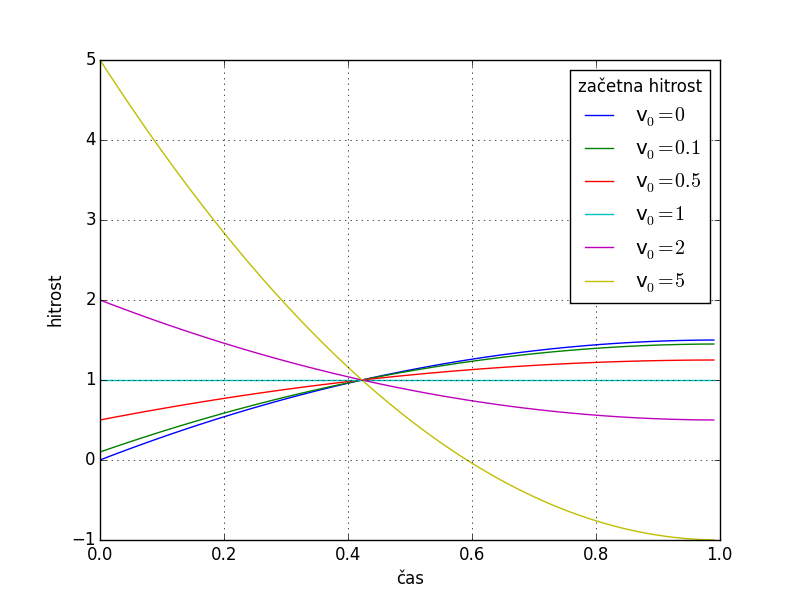
\includegraphics[scale=0.55]{slike/prva.png}
\caption[skica-EPR]{Primer rešitev za različne začetne hitrosti, po enačbi \ref{eq-v-ot-prva}}
\label{fig:prva}
\end{figure}
Za prepis problema v brezdimenzijsko obliko uporabimo naslednji zvezi, $T=\frac{t}{t_0}$ za čas, in $V(t)=v(t)\frac{t_0}{L_0}$ za hitrost. Te dve "transformaciji" vstavimo v rešitev diferencialne enačbe, ter še upoštevamo robne pogoje.

Za primer dinamičnih robnih pogojev/poljubni končni hitrosti, velja nasljednja zveza:
\begin{equation}
\label{eq-resitev-prva}
\frac{d \bar{L}}{d \dot{V}}\Big|_{T=1}=0
\end{equation}
Dobimo naslednja robna pogoja:
\begin{equation*}
\begin{aligned}
&V(0)=V_0\\
&\dot{V}(1)=0\\
\end{aligned}
\end{equation*}
Upoštevamo še pogoj:
\begin{equation}
\label{eq-norma}
\int_{0}^{1} V(t) dT=1
\end{equation}
in dobimo rešitve v obliki:
\begin{equation}
\label{eq-v-ot-prva}
V(T)=\frac{3}{2}T^2(V_0-1)+3T(1-V_0)+V_0
\end{equation}
Vidimo, da so rešitve parabole, edini parameter, ki vpliva na obliko gibanja, je le začetna hitrost. Različne oblike rešitev, pri nekaj različnih začetnih hitrostih se vidijo na sliki \ref{fig:prva}.





\section{Višje sode potence}

Oglejmo si primer, ko v funkcionalu izberemo višjo sodo potenco pospeška. Lagrangeova funkcija je potem:
\begin{equation}
\bar{L}=\dot{v}(t)^{2p}-\lambda v(t)
\end{equation}
Po uporabi E-L enačbe dobimo naslednjo diferencialno enačbo:
\begin{equation}
\ddot{v}(t)+\frac{\lambda}{2p(2p-1)}\dot{v}(t)^{-2p+2}=0
\end{equation}
Po dveh integracijah dobimo sledečo rešitev:
\begin{equation}
v(t)=(-\frac{\lambda}{2p})^{\frac{1}{2p-1}}(C_1+t)^{\frac{2p}{2p-1}}+C_2
\end{equation}
Po uporabi robnih pogojev, uporabi vezi ter vpeljavi brezdimenzijskih spremenljivk:
\begin{equation*}
\begin{aligned}
&v(0)=v_0\\
&\dot{v}(1)=0\\
\int_{0}^{1}& V(t) dT=1
\end{aligned}
\end{equation*}
pridemo do rešitve:
\begin{equation}
V(T)=\frac{4p-1}{2p}(1-V_0)(1-(1-T)^{\frac{2p}{2p-1}})+V_0
\end{equation}
Oglejmo si še limito, ko gre p proti neskončno. Takrat se enačba poenostavi v preprosto linearno funkcijo: $V(T)=2T(1-V_0)+V_0$. Linearno padanje/naraščanje hitrosto se dobro opazi pri p=10, medtem, ko pri p=5, pa krivulje malenkostno odstopajo od premice.




\begin{figure}[t]
\noindent\makebox[\textwidth][l]{%
\hspace{-\dimexpr\oddsidemargin+1in}%

\begin{minipage}[t]{0.5\paperwidth}
\begin{flushleft}

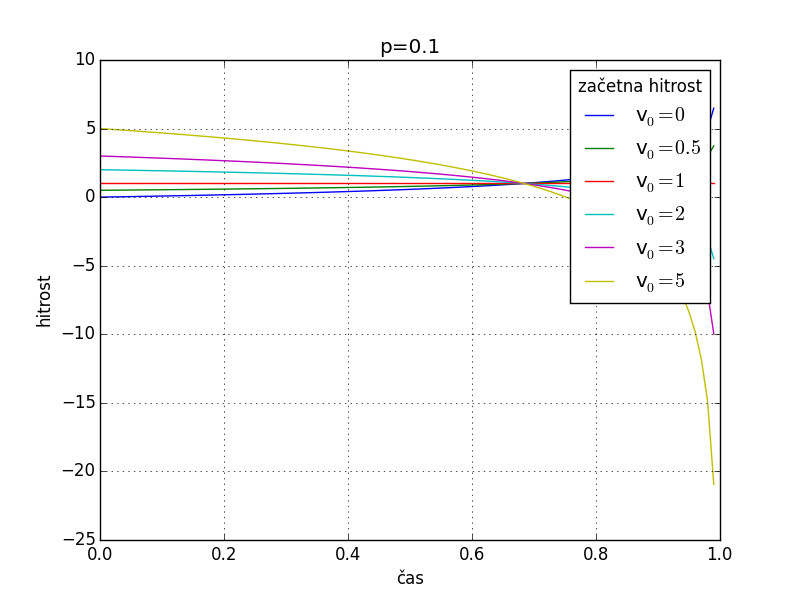
\includegraphics[scale=0.5]{slike/drugap=01.png}
\hspace{\fill}
\end{flushleft}
\end{minipage}
\begin{minipage}[t]{0.5\paperwidth}
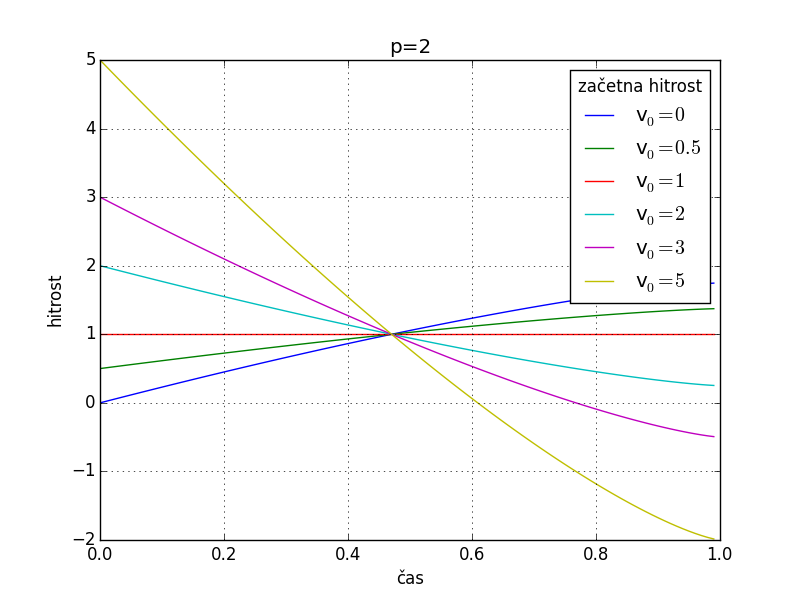
\includegraphics[scale=0.5]{slike/drugap=2.png}
\end{minipage}%
}
\noindent\makebox[\textwidth][l]{%
\hspace{-\dimexpr\oddsidemargin+1in}%

\begin{minipage}[t]{0.5\paperwidth}
\begin{flushleft}

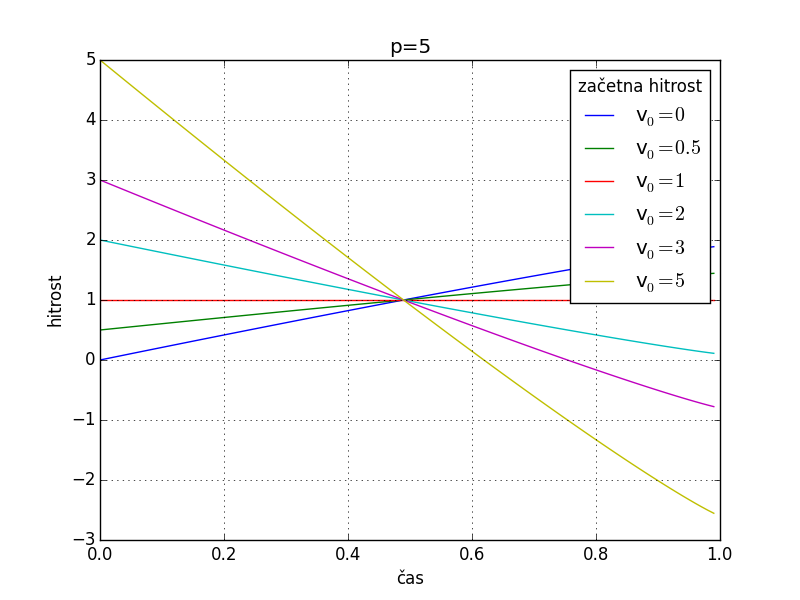
\includegraphics[scale=0.5]{slike/drugap=5.png}
\hspace{\fill}
\end{flushleft}
\end{minipage}
\begin{minipage}[t]{0.5\paperwidth}
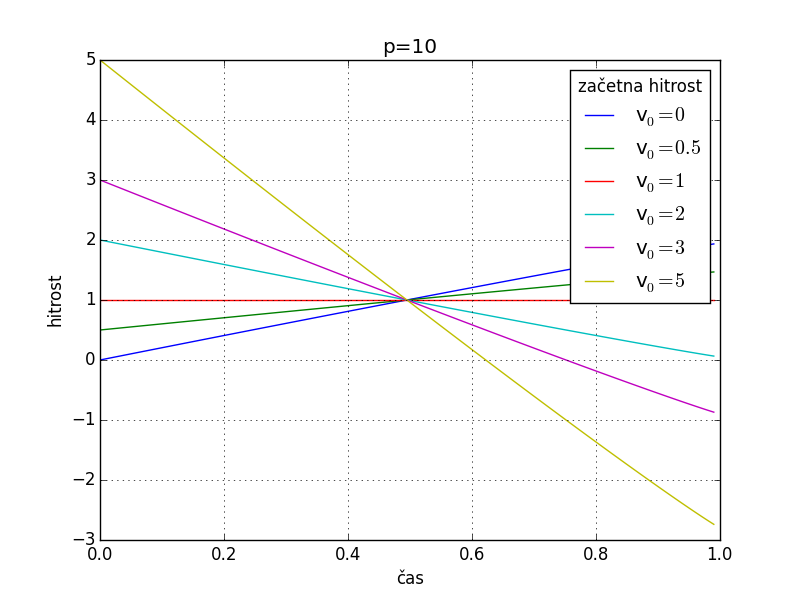
\includegraphics[scale=0.5]{slike/drugap=10.png}
\end{minipage}%
}
\caption{Primeri vožnje za različne potence pospeška.}
\end{figure}



\clearpage





\section{Prispevek kvadratičnega člena hitrosti}
Sedaj si bomo pogledali še kako vpliva kvadratični člen hitrosti v Lagrangeovi funkciji k našim rešitvam. Torej naša Lagrangeova funkcija je:
\begin{equation}
\bar{L}=\dot{v}(t)^2+Av(t)^2-\lambda v(t)
\end{equation}
Ko vstavimo to v E-L enačbo dobimo naslednjo diferencialno enačbo:
\begin{equation}
\ddot{v}(t)-Av(t)+\frac{\lambda}{2}=0
\end{equation}
ter njena rešitev:
\begin{equation}
v(t)=C_1 \sinh(\sqrt{A}t)+C_2 \cosh(\sqrt{A}t)+\frac{\lambda}{2C}
\end{equation}
Ob upoštevanju robnih pogojev (enaki kot v prejšnjih primerih), vezi in transformaciji spremenljivk, naslednjo enačbo:
\begin{equation}
V(T)=(V_0-AT_0\frac{1-V_0\frac{\tanh(\sqrt{A}T_0)}{\sqrt{A}T_0}}{1-\frac{\tanh(\sqrt{A}T_0)}{\sqrt{A}T_0}})(\cosh(\sqrt{A}T)-\tanh(\sqrt{A}T_0)\sinh(\sqrt{A}T))+AT_0\frac{1-V_0\frac{\tanh(\sqrt{A}T_0)}{\sqrt{A}T_0}}{1-\frac{\tanh(\sqrt{A}T_0)}{\sqrt{A}T_0}}
\end{equation}
Ker enačba ni pretirano lepa in se ne vidi njenih lastnosti si oglejmo grafe za nakaj vrednosti začetne hitrosti in pri različnih vrednsoti konstante A. Opazimo, da z naraščanjem vredosti konstante A, se hitrost hitreje približuje h povprečni vrednosti vožnje.


\begin{figure}[t]
\noindent\makebox[\textwidth][l]{%
\hspace{-\dimexpr\oddsidemargin+1in}%

\begin{minipage}[t]{0.5\paperwidth}
\begin{flushleft}

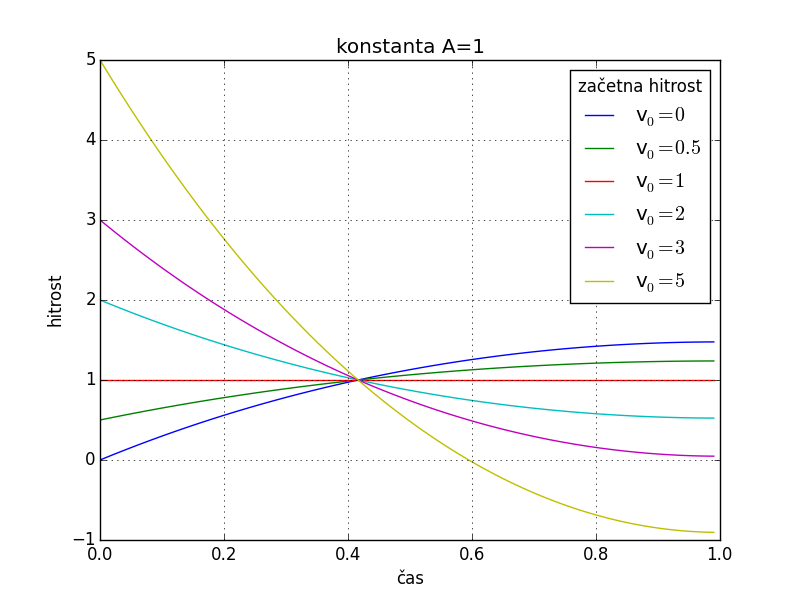
\includegraphics[scale=0.5]{slike/konstanta1.png}
\hspace{\fill}
\end{flushleft}
\end{minipage}
\begin{minipage}[t]{0.5\paperwidth}
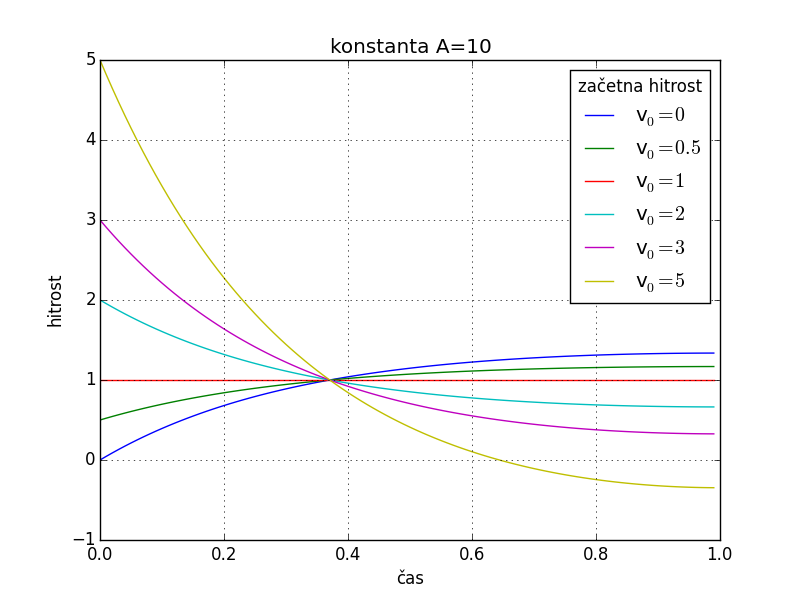
\includegraphics[scale=0.5]{slike/konstanta10.png}
\end{minipage}%
}
\noindent\makebox[\textwidth][l]{%
\hspace{-\dimexpr\oddsidemargin+1in}%

\begin{minipage}[t]{0.5\paperwidth}
\begin{flushleft}

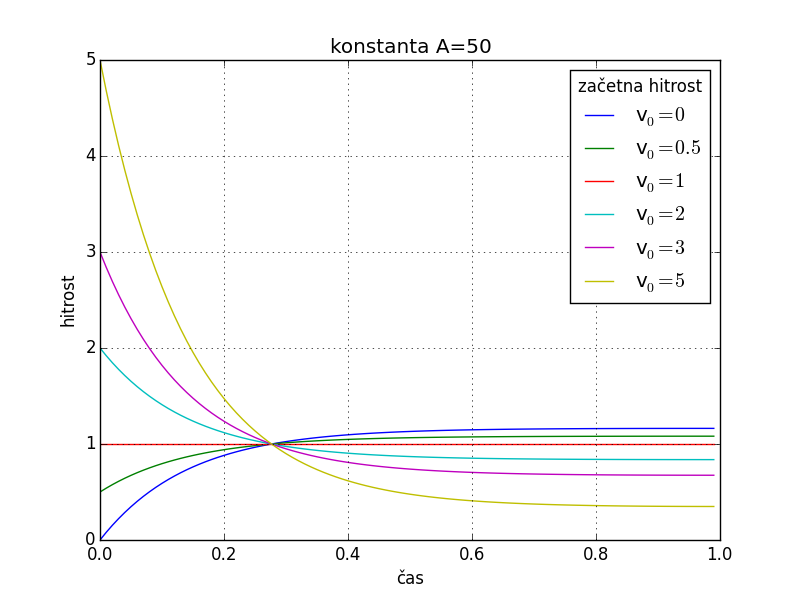
\includegraphics[scale=0.5]{slike/konstanta50.png}
\hspace{\fill}
\end{flushleft}
\end{minipage}
\begin{minipage}[t]{0.5\paperwidth}
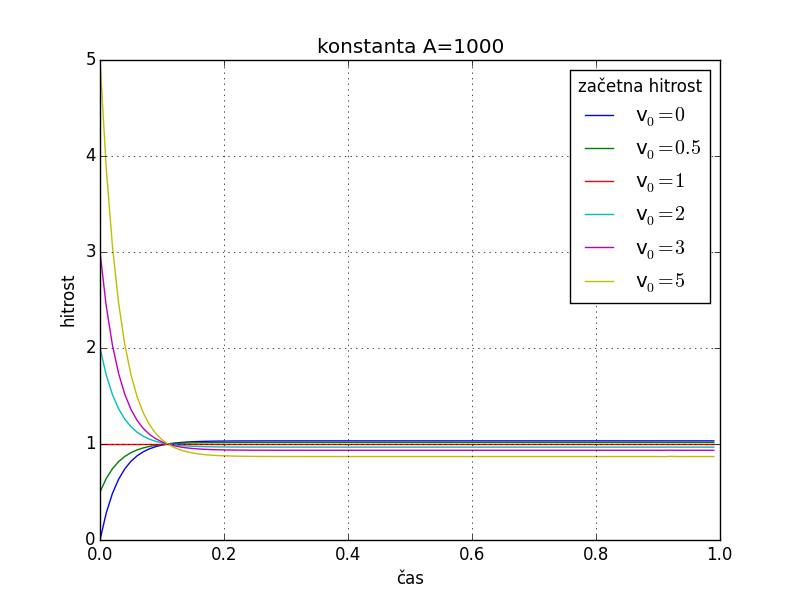
\includegraphics[scale=0.5]{slike/konstanta1000.png}
\end{minipage}%
}
\caption{Primeri vožnje za različne vrednosti konstante A.}
\end{figure}


\clearpage





\section{Periodična rešitev}
Oglejmo si primer rešitve diferencialne enačbe \ref{eq-osnovna}, z naslednjima robnima pogojema:
\begin{equation*}
\begin{aligned}
v(0)=v_0\\
v(t_0)=v_0
\end{aligned}
\end{equation*}
Dobimo rešitev:
\begin{equation}
V(T)=-6(1-V_0)T^2+6(1-V_0)T+V_0
\end{equation}

\begin{figure}[h]
%\centering
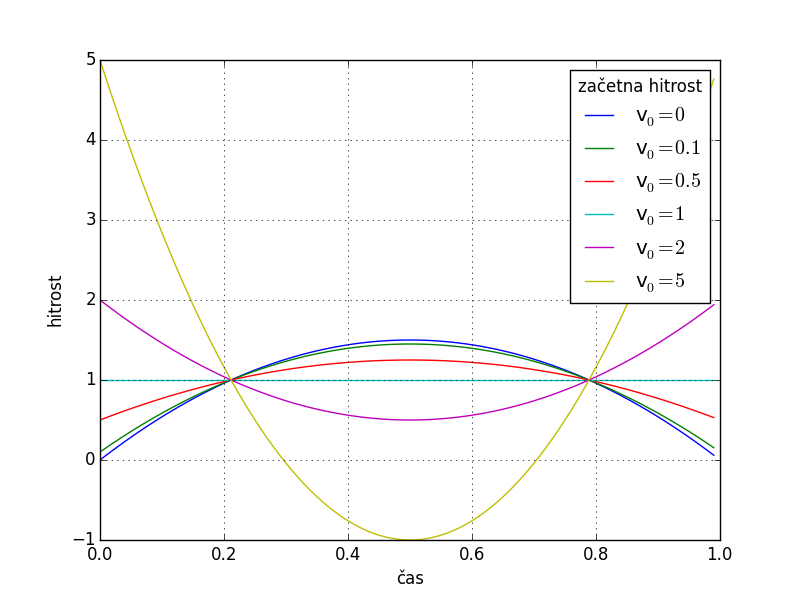
\includegraphics[scale=0.6]{slike/cetrta.png}
\caption{Primer rešitev za različne začetne hitrosti, za enačbo \ref{eq-osnovna}, za primer enake končne in začetne hitrosti.}
\label{fig:prva}
\end{figure}

\pagebreak

%
%\cite{pub265}
%\cite{kragh2002quantum}
%\cite{PhysRevFocus.16.10}
%\cite{fizika3}
%\cite{schwabl2007quantum}


%\bibliographystyle{plain}
%\bibliography{seminar}


%\listoffigures

%----------------------------------------------------------------------------------------

\end{document}
				